% ----------------------------------------------------------
% Introdução (exemplo de capítulo sem numeração, mas presente no Sumário)
% ----------------------------------------------------------
\chapter[Introdução]{Introdução}
%\addcontentsline{toc}{chapter}{Introdução}
% ----------------------------------------------------------

 A siderurgia é o processo de transformar ferro, sucata, carbono e fundentes (\textit{e.g.} calcário e dolomita) em aço. Existem dois tipos de usinas siderúrgicas: (i) a usina simples que só utiliza como matéria prima o carvão mineral; (ii) a usina integrada que utiliza tanto o carvão mineral como o carvão vegetal em sua produção.
 
 O processo se inicia na Coqueria com a transformação do minério em pelotas e a destilação do carvão, para obtenção do coque, dele se obtendo ainda subprodutos carboquímicos.
%
 Nas usinas integradas há um processo adicional que é a Sinterização que tem como produto da aglomeração a quente do minério de ferro, fundentes e finos de coque, o sínter.
%
 O coque e o sínter são levado aos Alto-Fornos, cuja a temperatura é cerca de 1.500ºC, o ferro se liquefaz e passa a ser chamado de ferro gusa que é levado por carros torpedos para a aciaria onde ocorrerá o refino através da queima de impurezas e adições.
  
A transformação do ferro-gusa em aço acontece na Aciaria, através da oxidação dos elementos do gusa que se deseja mitigar, como o carbono, silício, fósforo e enxofre. O produto da Aciaria é o aço líquido.

 O aço líquido é encaminhado para o Lingotamento Contínuo que, em processo de solidificação, é deformado mecanicamente e transformado em produtos siderúrgicos utilizados pela indústria de transformação, como tarugos, bobinas, arames etc. \cite{aco}

 \begin{figure}[htbp]
	\centering
	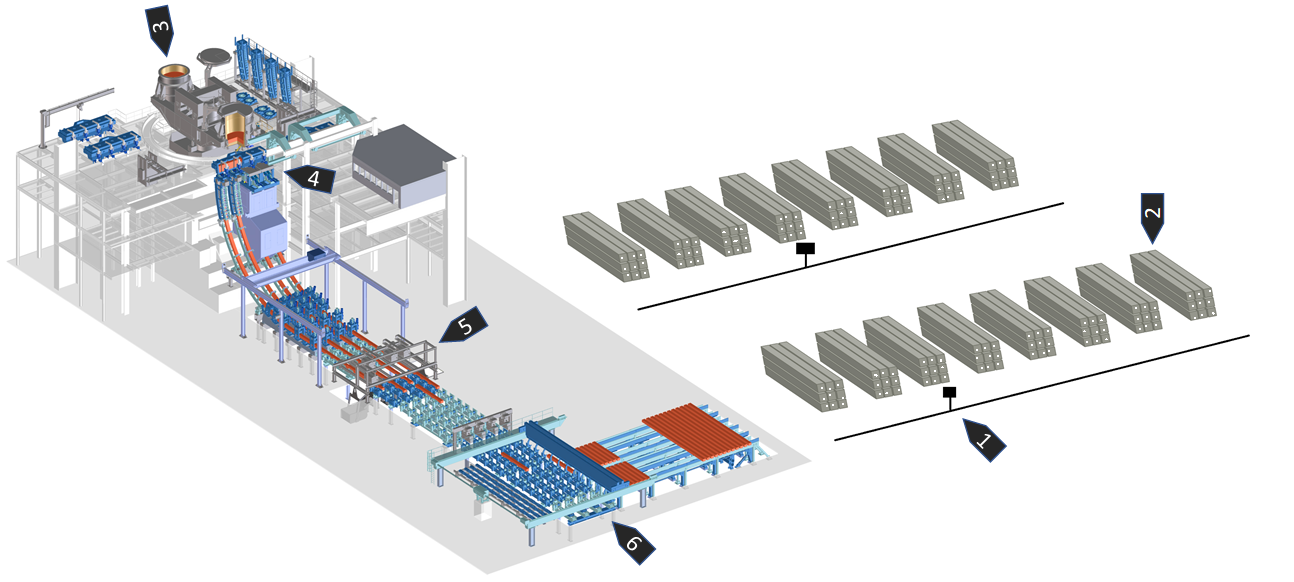
\includegraphics[width=1.1\linewidth]{figuras/Steel/process.png}
	\caption{Processo de lingotamento Contínuo de Tarugos}
	\legend{Fonte: \citeauthor{freitas2013analise} (\citeyear{freitas2013analise})}
	\begin{tabular}{r@{: }l r@{: }l}
        1 & Câmera Fotográfica & 4 & Molde \\
        2& Pilha de corridas & 5 & Máquina de Oxicorte \\
        3 & Panela de aço& 6 & Transferidor de tarugos \\
    \end{tabular}
	\label{fig:processLing}
\end{figure}

Especificamente na usina da Gerdau em Ouro Branco (Minas Gerais), o processo de lingotamento consiste no despejamento de uma panela com $\sim~224$ toneladas de aço, a uma temperatura de $\sim~1550~$ºC, no distribuidor que precede o lingotamento em si (Figura \ref{fig:processLing}).
%
Este processo pode levar de horas a dias sem interrupção.
%
A cada batelada da panela da-se o nome de \textbf{corrida}.


A etapa de solidificação ocorre de fora para dentro do veio
%
\footnote{\textit{Veio} é o nome que se dá ao conjunto formado pelo molde, a máquina Oxicorte e os rolos de extração e endireitadores. Quanto maior o número de veios, maior a produtividade da máquina, mas mais complexo se torna o seu controle.} 
%
em função do contato com as paredes refrigeradas do molde, aspersão de água em \textit{sprays} e perda de calor por radiação para o ambiente. Essa troca de calor faz com que o aço se solidifique gradativamente criando zonas onde o material pode ser encontrado ao mesmo tempo em seus estados sólido na parte exterior e líquido no interior (Figura \ref{fig:processLingSolid}).

\begin{figure}[hbt!]
	\centering
	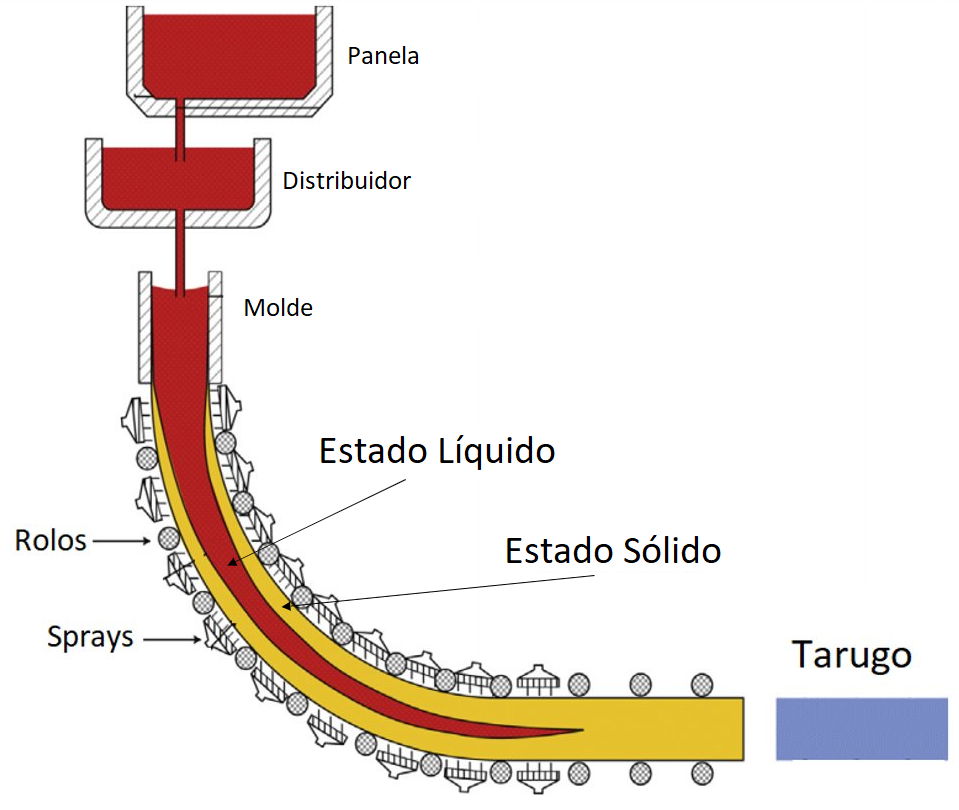
\includegraphics[width=0.8\linewidth]{figuras/Steel/estadoSolidoLiq.png}
	\caption{Estados do aço no processo de lingotamento contínuo}
	\legend{Fonte: \citeauthor{YU201736} (\citeyear{YU201736})}
	\label{fig:processLingSolid}
\end{figure}

No processo final de cada corrida, os tarugos são cortados na máquina Oxicorte \footnote{Corta o tarugo em um tamanho previamente definido, possibilitando assim o seu trasporte até a sua destinação final.} de modo que a sessão transversal de casa um seja quadrada, como mostrado na Figura \ref{fig:processLing}.  

Os tamanhos dos cortes são feitos de acordo com a demanda do cliente e origina em média 100 tarugos. O número de tarugos que depende do diâmetro das peças que podem ser 130mm ou 160mm e do comprimento das mesmas que variam de 07 a 14m. Todas as peças de uma mesma corrida têm o mesmo diâmetro e comprimento. Após serem cortados, os tarugos são transportados para o despacho por uma ponte rolante a base de eletroímãs que suportam altas temperaturas e $27$ toneladas de carga. 


\begin{figure}[htbp]
	\centering
	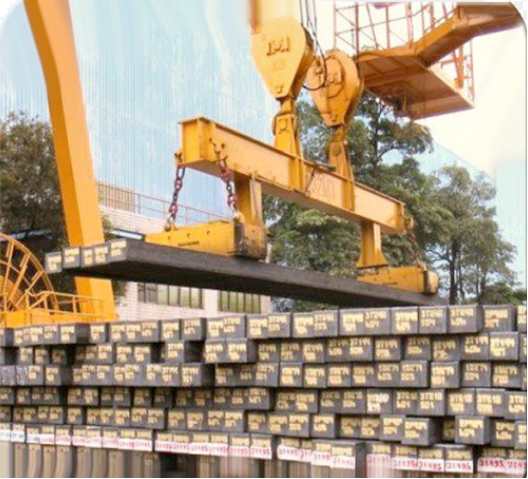
\includegraphics[width=0.7\linewidth]{figuras/Steel/ponte_rolante.png}
	\caption{Ponte Rolante}
	\legend{Fonte: \citeauthor{ponte-rolante} (\citeyear{ponte-rolante})}
	\label{fig:crane}
\end{figure}

\begin{figure}[htbp]
	\centering
	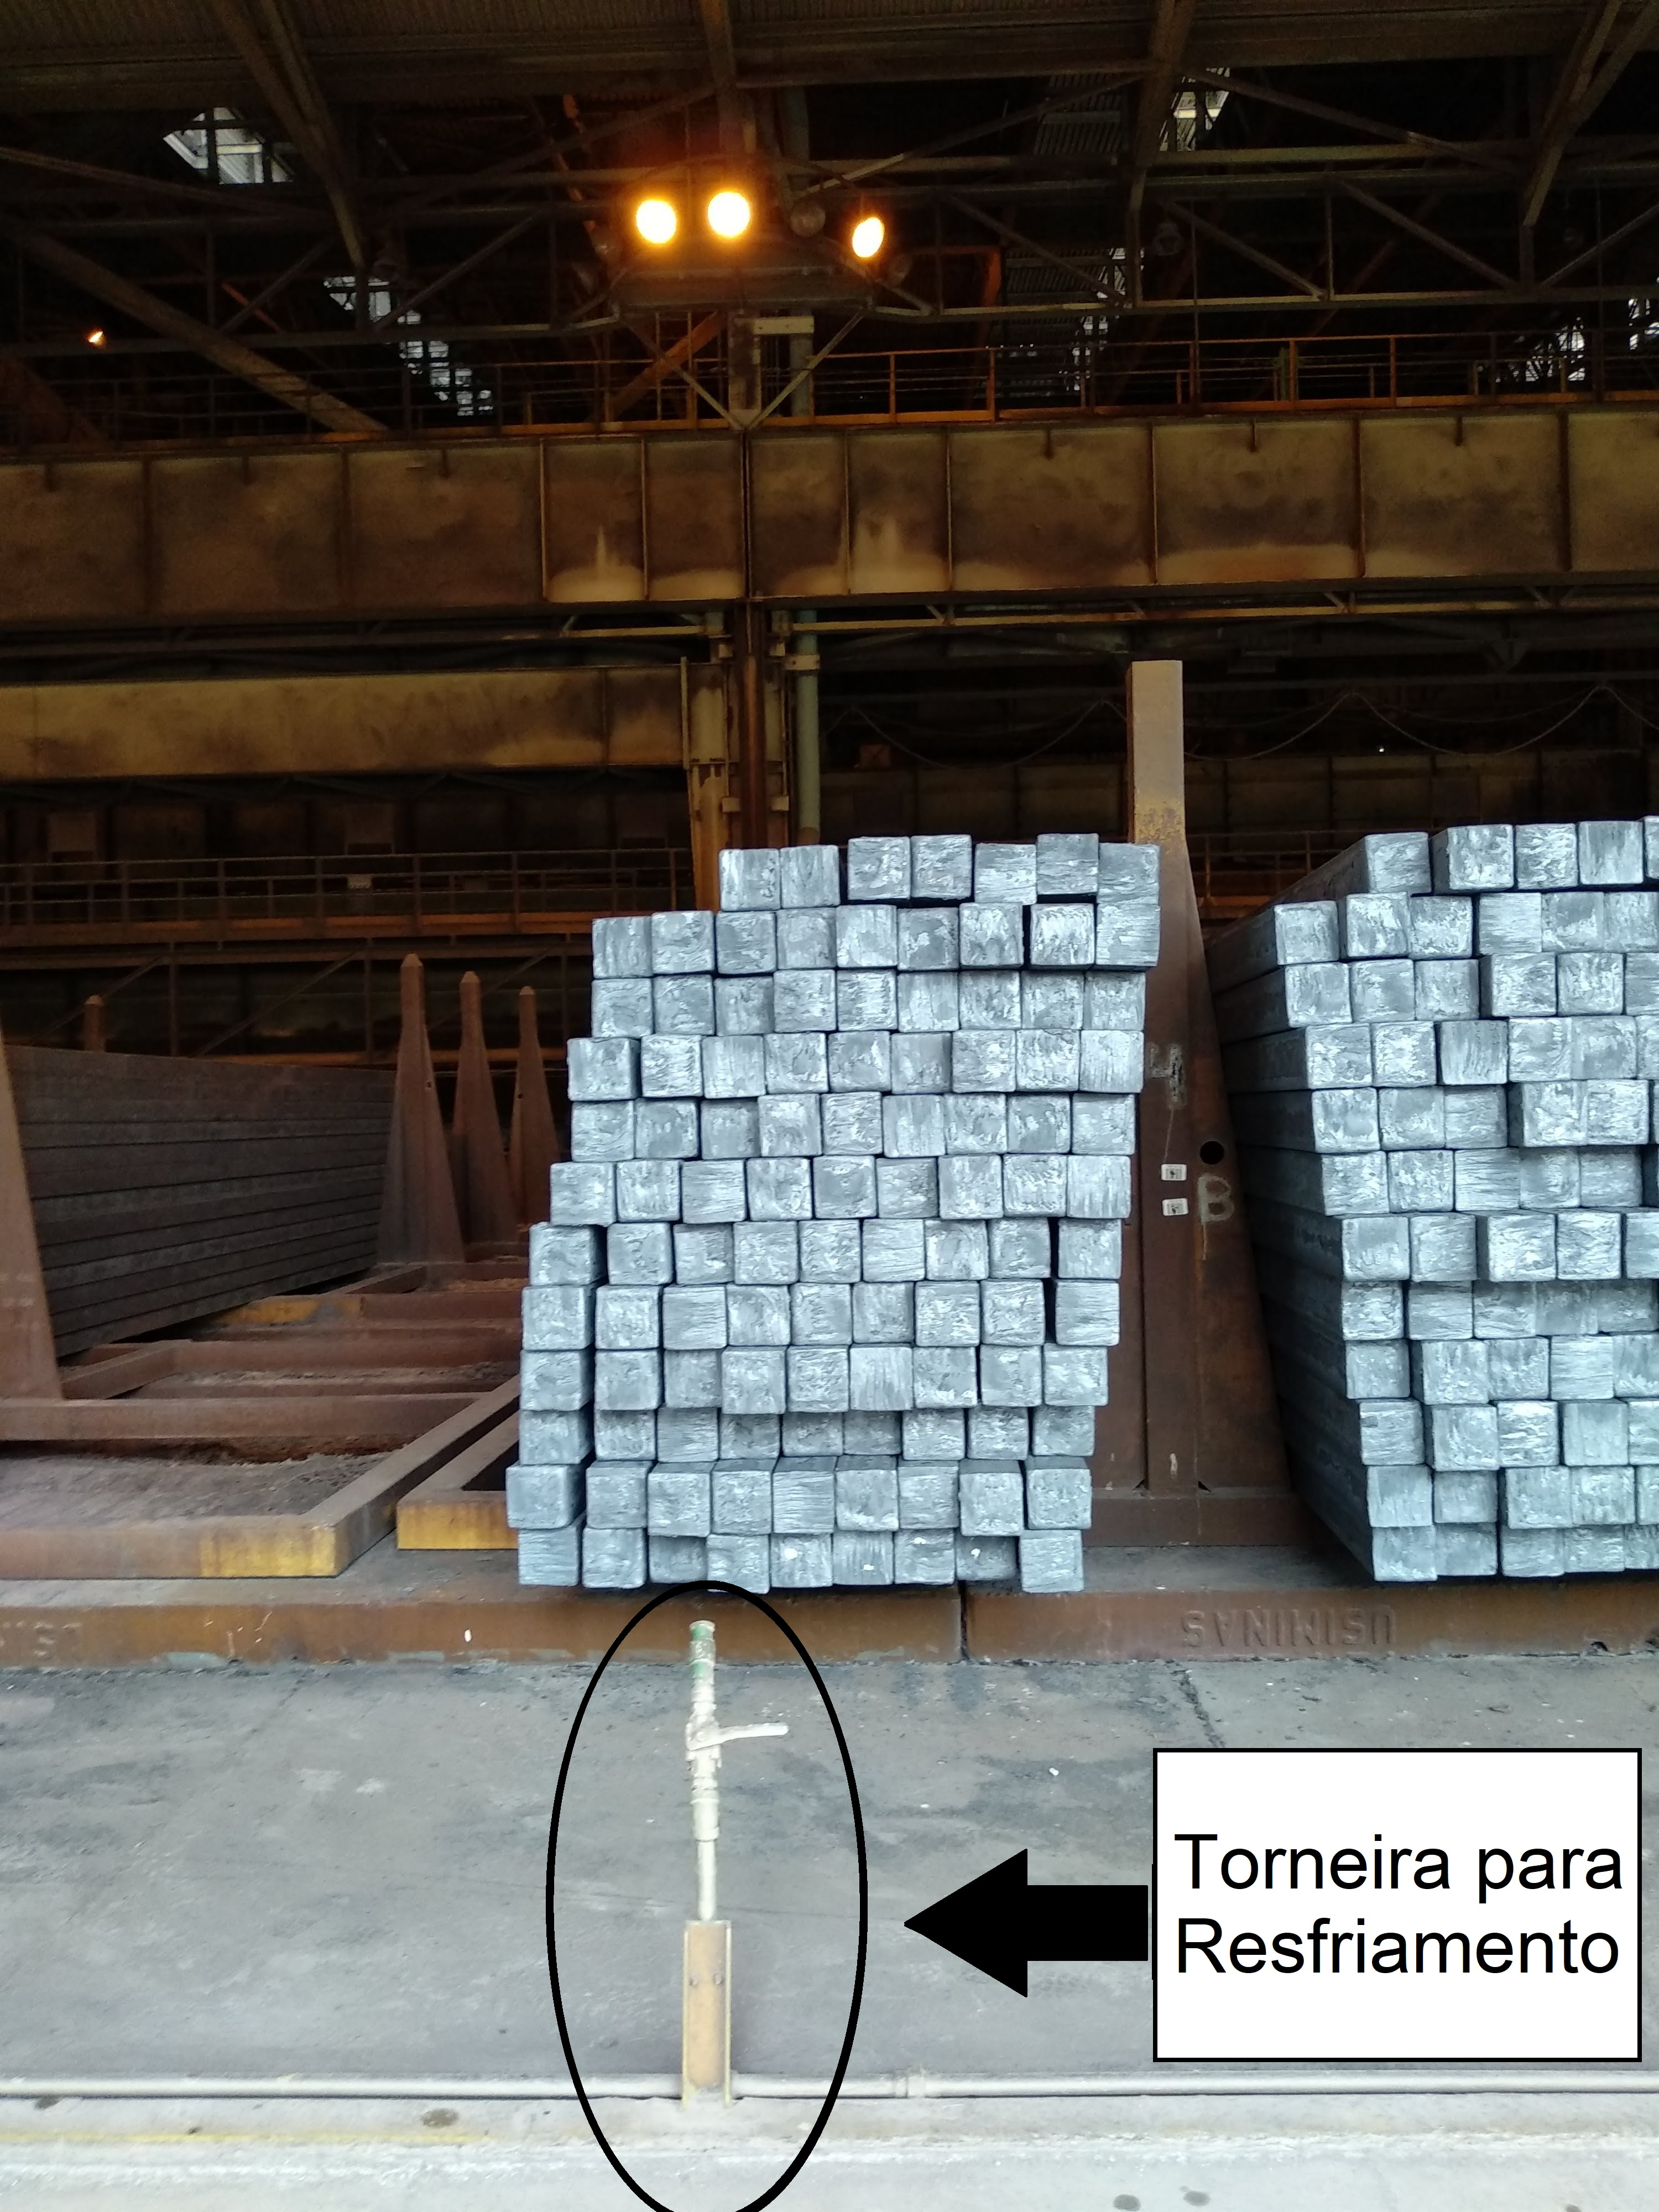
\includegraphics[width=0.5\linewidth]{figuras/Steel/despacho.jpg}
	\caption{Despacho}
	\label{fig:despacho}
\end{figure}

Os tarugos vão para a zona de despacho a uma temperatura de $\sim~700$ºC.
%
Após cerca de 20 horas, a temperatura cai para $150~$ºC, temperatura adequada para a fixação das etiquetas de identificação dos tarugos.
%
Um jato de água é direcionado aos tarugos para acelerar o resfriamento (Figura \ref{fig:despacho}) com frequência constante apenas na parte frontal.
%
A eventual injeção de água no centro do tarugo pode empenar a peça, uma vez que a temperatura central do tarugo está mais quente que as extremidades.


Após o tempo necessário, o operador prega as etiquetas utilizando Silicone Acético Transparente, no qual foi testada e comprovada sua eficácia na resistência sobre alta temperatura.

\begin{figure}[htbp]
	\centering
	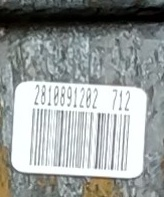
\includegraphics[width=0.25\linewidth]{figuras/Steel/barcode.jpg}
	\caption{Etiqueta}
	\label{fig:barcode}
\end{figure}

A rotulação é importante pois evita a mistura de aço entre uma corrida e outra, viabiliza a rastreabilidade e identificação do aço em processos posteriores como, por exemplo, na laminação até o cliente final. 
%A composição dos números intrínsecos ao código de barra impresso na etiqueta metálica, como da Figura \ref{fig:barcode}, é o que permite a identificação supracitada a saber:

\begin{table}[]
	\centering
	\begin{tabular}{|l|l|}
		\hline
		\rowcolor[HTML]{ECF4FF} 
		\multicolumn{1}{|c|}{\cellcolor[HTML]{ECF4FF}Número} & \multicolumn{1}{c|}{\cellcolor[HTML]{ECF4FF}2810891202 712}\\ \hline
		28 & Número do convertedor que pode ser CV1 (27) ou CV2 (28).\\ \hline
		108912 & Adicionando o convertedor a este número, forma-se o número da corrida no qual: 
    		    \cr & CV2 = 2 e CV1 = 1, temos
    		    \cr & Número da corrida: 2108912\\ \hline
        02 & 02 é a rota que a panela passou no lingotamento. Ou seja, 02 = tarugo.\\ \hline
        712 & Número 7 é o veio que a peça foi lingotada e 12 o número da peça.\\ \hline
	\end{tabular}
	\caption{Significado dos dígitos da etiqueta de rotulação.}
	\label{tab:tag}
\end{table}

O número de identificação da etiqueta pode ser reconhecido pelos dígitos ou pelo código de barras através de um leitor de código de barras à \textit{laser}. Em cada etiqueta, o código de barras e os dígitos acima deste correspondem à mesma sequência numérica.

Os atuais problemas na identificação das etiquetas são: 
\begin{enumerate}
	\item O processo é atualmente manual e demorado.
	\item O local em que a pilha de peças se encontra é perigoso devido ao fato de, a todo momento, uma ponte rolante estar trabalhando no mesmo local.
\end{enumerate}

\section{Revisão bibliográfica} 

% TODO Aqui é o momento ideal pra aparecer uns 2/3 parágrafos de revisão bibliográfica hein kkk Cite dos esforços em automatizar o processo (se houve) e o que outros autores já fizeram em áreas similares. :)

\section{Objetivos} 

Desenvolver um sistema automático para a identificação robusta e geração de relatório para cada corrida.

Através de uma foto, o sistema será capaz de identificar as etiquetas fixadas no Tarugo, contar o número de etiquetas, identificar o código de barras e, além disso, identificar os números que se encontram acima do mesmo.

Será criado uma aplicação Web com um servidor para que seja gerado um relatório detalhado de forma automática facilitando a conferência por parte do operador.

\subsection{Objetivos específicos}

\begin{itemize}
	\item Recolher várias imagens contendo todos os Tarugos;
	\item Implementar o sistema de expansão dos \textit{datasets} através do método \textit{Data Augmentation}, para que a quantidade de imagens seja suficiente para treinar os modelos de \textit{Machine Learning};
	\item Treinar e implementar o modelo de reconhecimento de código de barras;
	\item Treinar e implementar o modelo de reconhecimento de números;
	\item Implementar a aplicação Web;
	\item Publicar a aplicação no Google Cloud Plataform;
	\item Integrar todos os sistemas a fim de garantir as funcionalidades do projeto;
	\item Executar os procedimentos em ambiente online a fim de validar o projeto;
\end{itemize}

%\section{Justificativas e Relev{\^a}ncia}

\section{Organização do trabalho}

O presente trabalho está organizado em 5 capítulos. No Capítulo 1, encontra-se
a apresentação do problema e suas possíveis soluções, além de apresentar os objetivos
propostos.

O Capítulo 2 consiste nas definições e nas explicações das linguagens de programação, dos métodos e dos \textit{softwares} utilizados no projeto.

No Capítulo 3 é apresentado a estrutura geral do sistema, a metodologia em que foi construído. Explica-se também as etapas do desenvolvimento e códigos implementados.

O Capítulo 4 trata dos experimentos realizados no sistema e seus resultados.

No Capítulo 5 são abordadas as considerações finais do trabalho.